% if you want the answers to appear uncomment the below
\documentclass[answers]{exam}
% otherwise uncomment the below
%\documentclass{exam}

\usepackage{graphicx}
\usepackage[letterpaper, margin=.9in]{geometry}
\usepackage{natbib}
\bibpunct{(}{)}{;}{a}{,}{,}
\usepackage{url}
\def\UrlFont{\rm}

\usepackage[utf8x]{inputenc}
\usepackage{array}
\usepackage{verbatim}
\usepackage{amsfonts}
\usepackage{amsmath}
\setlength{\parskip}{2ex} 

% Cannot place floats in figure environment.
\usepackage{caption}
\usepackage{newfloat}
%\DeclareCaptionListFormat{myliststyle}{#1.#2}
\DeclareCaptionType{mytype}[Solution Fig.][List of mytype]
\newenvironment{myfigure}{\captionsetup{type=mytype}}{}



\newenvironment{packed_enum}{
\begin{enumerate}
 \setlength{\itemsep}{0pt}
  \setlength{\parskip}{0pt}
  \setlength{\parsep}{0pt}
}{\end{enumerate}}
\newenvironment{packed_item}{
\begin{itemize}
 \setlength{\itemsep}{0pt}
  \setlength{\parskip}{0pt}
  \setlength{\parsep}{0pt}
}{\end{itemize}}

 \newcommand\independent{\protect\mathpalette{\protect\independenT}{\perp}}
    \def\independenT#1#2{\mathrel{\setbox0\hbox{$#1#2$}%
    \copy0\kern-\wd0\mkern4mu\box0}} 


\bibliographystyle{plainnat}

\pagestyle{myheadings}
\markright{Advanced Topics in Causal Inference \hfill  R Lab \#0 \hfill}


\title{R Lab 0 - \texttt{R} Programming Refresher}
\author{Advanced Topics in Causal Inference}
\date{}

\usepackage{Sweave}
\begin{document}
\Sconcordance{concordance:RLab0_answers.tex:RLab0_answers.Rnw:%
1 56 1 1 0 47 1 1 2 4 0 2 2 7 0 2 2 1 0 1 1 6 0 2 2 1 0 1 1 6 0 1 2 12 %
1 1 3 5 0 1 4 5 0 1 4 5 0 1 4 8 0 1 4 7 0 1 2 6 0 1 1 6 0 1 2 5 1 1 3 5 %
0 1 2 2 1 1 3 2 0 1 3 10 0 1 3 3 1 9 0 1 3 3 1 1 2 1 0 1 1 3 0 1 2 1 1 %
1 2 4 0 1 2 4 1 1 2 7 0 1 2 3 1 1 2 7 0 1 2 5 1 1 2 1 0 1 1 7 0 1 2 1 1 %
1 2 8 0 1 2 4 1 1 2 7 0 2 2 7 0 1 2 2 1 1 2 8 0 1 2 11 1 1 3 9 0 1 4 9 %
0 1 4 2 0 1 1 7 0 1 2 3 1 1 2 1 0 1 2 1 1 1 2 1 1 1 2 1 1 3 0 1 2 6 1 1 %
2 4 0 2 2 1 0 1 1 11 0 2 2 7 0 1 2 1 1 1 2 7 0 1 2 1 1 1 2 7 0 1 2 23 1 %
1 3 8 0 1 4 2 0 1 1 3 0 1 2 4 1 1 2 4 0 2 2 4 0 2 2 7 0 2 2 6 0 1 2 11 %
0 1 2 12 0 1 2 2 1 1 2 6 0 1 1 5 0 1 1 6 0 1 2 11 1 1 3 8 0 1 2 1 3 6 0 %
1 2 1 5 8 0 1 2 5 1 1 7 9 0 1 2 2 1 1 2 7 0 1 2 17 1 1 9 11 0 1 2 30 1 %
1 3 5 0 1 8 9 0 1 23 24 0 1 4 5 0 1 4 13 0 1 1 12 0 1 2 23 1 1 2 1 0 2 %
1 4 0 1 2 19 1 1 2 4 0 2 2 4 0 1 2 5 1 1 2 4 0 2 2 4 0 2 2 4 0 1 2 10 1 %
1 2 4 0 2 2 4 0 1 2 14 1 1 3 2 0 2 1 3 0 1 4 5 0 1 4 5 0 1 4 2 0 2 1 3 %
0 1 4 5 0 1 4 5 0 1 2 3 1 1 3 5 0 1 5 3 0 1 2 1 0 1 2 4 0 1 5 6 0 1 4 5 %
0 1 4 5 0 1 5 3 0 1 2 4 0 1 5 3 0 1 1 1 2 11 0 1 2 4 0 1 6 4 0 1 2 1 0 %
1 2 5 0 1 1 5 0 1 1 22 0 1 1 16 0 1 2 9 1}

\maketitle



\noindent \textbf{Goals for this lab:} \\ 
1. Review of \texttt{R} programming and good programming practice. \\
2. Create a basic function to generate data with $O = (W, A, Y)$ structure. \\
3. Implement g-computation, IPTW, and TMLE estimators inspired by the average treatment effect (ATE) of a point treatment intervention. \\

\noindent \textbf{Next lab:} \\
1. Explore different data structures, inspired by real-world experiments. \\
2. Simulate data generating process that gives rise to the data we observe. \\
3. Think of studies in which these data generating systems may occur.\\

\section{Introduction and Motivation}

Welcome to Advanced Topics in Causal Inference \texttt{R} Labs! This semester we'll be working in \texttt{R} to implement concepts we've learned in lectures and discussion sections. In this lab we'll provide a refresher of \texttt{R} programming. Here is a link to cheatsheets I find useful that you may enjoy studying on your own: https://www.rstudio.com/resources/cheatsheets/.

\noindent Section 2 will give you a refresher on \texttt{R} basics, including objects, subsetting, making plots, etc. Section 3 will walk you through how to generate data, and Section 4 will implement the 3 estimators we learned in Causal I to estimate the average treatment effect. You won't be turning in this lab, so feel free to complete as many or few sections as you feel will help you get a solid foundation before we start labs (to turn in) next week.

\noindent In future labs, please turn in relevant \texttt{R} code, text, and figures. Consider turning in your homework as a compiled \texttt{R} Markdown (RMD) file, which ``knits" your code, text, and figures into a single PDF, Word, or html document. A .Rmd template with further instructions can be found on bCourses.

\begin{figure}
\begin{center}

\includegraphics[width=.4\textwidth]{welcome.jpg}
\caption{Welcome to Causal II labs!}
\end{center}
\end{figure}

\section{\texttt{R} review and refresher}
\subsection{Help files}

Help files in \texttt{R} are extremely useful. Coding in \texttt{R} isn't so much about memorizing functions; it's more useful to know how to look up commands. Knowing how to read the help documentation will make you a much more independent and creative programmer. 

\noindent For example, type \texttt{?rnorm} in your console in the command line. This pulls up the help page for the \texttt{rnorm()} function. What does the function \texttt{rnorm()} do? The help file gives you a description of all things having to do with the normal distribution (you will see a few other functions listed, such as \texttt{pnorm()}, \texttt{dnorm()}, and \texttt{qnorm())}.

\noindent The \textit{Usage} section lets you know what arguments go into which functions. If there's an equal sign (i.e., =), that means that argument has a default value, so you don't need to specify that argument. You only need to specify if you want something different than the default. 

\noindent The \textit{Arguments} section describes what each of the arguments are. 

\noindent So, for example, \texttt{rnorm(n = 3, mean = 4, sd = 1)} generates 3 random numbers from a normal distribution with mean 4 and standard deviation 1. And \texttt{rnorm(n = 3)} generates 3 random numbers from a normal distribution with mean 0 and standard deviation 1. Notice we don't need to specify the \texttt{mean} and \texttt{sd} arguments in \texttt{rnorm()} if we want to generate numbers from a $Normal(\mu = 0, \sigma = 1)$ distribution because these are the default parameters (i.e., in the Usage section of the help file, the arguments \texttt{mean} and \texttt{sd} are equal to 0 and 1, respectively). Conversely, we always need to specify what \texttt{n} is because there's no default (i.e., no '=' sign after \texttt{n}).


\subsection{Assigning values to \texttt{R} objects}

We can assign results of computations to variables. Type each of the following lines either in an \texttt{R} script (and run each line), or in your console:
\begin{Schunk}
\begin{Sinput}
> x = (6-2)^.5/3^2
\end{Sinput}
\end{Schunk}
Here we are assigning a complicated arithmetic computation to the variable \texttt{x}. Notice what comes up in the workspace window when you assign the variable \texttt{x} to that value. Notice what comes up in the console when you run \texttt{x}:
\begin{Schunk}
\begin{Sinput}
> x
\end{Sinput}
\begin{Soutput}
[1] 0.2222222
\end{Soutput}
\end{Schunk}
\texttt{identical()} is a function that outputs a logical vector telling us whether two variables are identical:
\begin{Schunk}
\begin{Sinput}
> X = 3 
> identical(x, X)  
\end{Sinput}
\begin{Soutput}
[1] FALSE
\end{Soutput}
\end{Schunk}
As you can see here: \texttt{R} is case sensitive! Here we're catenating \texttt{x} and \texttt{X} into a vector called \texttt{y}:
\begin{Schunk}
\begin{Sinput}
> y = c(x, X)  
> y
\end{Sinput}
\begin{Soutput}
[1] 0.2222222 3.0000000
\end{Soutput}
\end{Schunk}

\noindent\textbf{On your own} (remember, use \texttt{?} to figure out what a function does and what arguments that go into a function):

\begin{enumerate}
\item Use the \texttt{rep()} function to make a vector that repeats the number ``4" 5 times (i.e., 4 4 4 4 4). Assign that vector to the variable \texttt{z}.
\item Use the \texttt{seq()} function to make a vector that shows odd numbers from 1 to 10 (i.e., 1 3 5 7 9). Assign that vector to the variable \texttt{y}. Notice how we've overwritten the variable \texttt{y} we had before.
\item Use the \texttt{sample()} function to sample 17 of elements from \texttt{y} with replacement. Assign that vector to the variable \texttt{w}. 
\item Add \texttt{z + y}.
\item Add \texttt{y + w}. What happened? Why? (Hint: use the \texttt{length()} function on \texttt{y} and \texttt{w}).
\item Remove \texttt{w} using the \texttt{rm()} function.
\end{enumerate}

\begin{solution}
\begin{Schunk}
\begin{Sinput}
> #1. use the rep() function to make vector z
> z = rep(x = 4, times = 5)
\end{Sinput}
\end{Schunk}
\begin{Schunk}
\begin{Sinput}
> #2. use seq() function to make vector y
> y = seq(from = 1, to = 10, by = 2)
\end{Sinput}
\end{Schunk}
\begin{Schunk}
\begin{Sinput}
> #3. use sample() function to make vector W
> w = sample(x = y, size = 17, replace = TRUE)
\end{Sinput}
\end{Schunk}
\begin{Schunk}
\begin{Sinput}
> #4. add z + y
> z + y
\end{Sinput}
\begin{Soutput}
[1]  5  7  9 11 13
\end{Soutput}
\end{Schunk}
\begin{Schunk}
\begin{Sinput}
> #5. add y + w
> y + w
\end{Sinput}
\begin{Soutput}
 [1]  6  4 12  8 14  4  8  8 12 18  2 10  6 16 16  6  4
\end{Soutput}
\begin{Sinput}
> # why did we get a warning?
> length(y)
\end{Sinput}
\begin{Soutput}
[1] 5
\end{Soutput}
\begin{Sinput}
> length(w)
\end{Sinput}
\begin{Soutput}
[1] 17
\end{Soutput}
\end{Schunk}


\noindent The vectors \texttt{y} and \texttt{w} do not have the same length (in contrast to question 4). In cases like these, \texttt{R} recycles the \texttt{y} vector for the remaining elements of the vector \texttt{w}. 

\noindent If \texttt{w} had been a multiple of \texttt{y} (for example, if \texttt{w} was 20), we wouldn't have gotten a warning message - beware of recycling!

\begin{Schunk}
\begin{Sinput}
> #6. remove the variable w
> rm(w)
\end{Sinput}
\end{Schunk}

\end{solution}

\begin{Schunk}
\begin{Sinput}
> #7. other example uses
> n_items <- 4
> for (i in seq(n_items)) {
+   print(paste(i, "bat, mwahaha"))
+ }
\end{Sinput}
\begin{Soutput}
[1] "1 bat, mwahaha"
[1] "2 bat, mwahaha"
[1] "3 bat, mwahaha"
[1] "4 bat, mwahaha"
\end{Soutput}
\begin{Sinput}
> die = 1:6
> manyRolls = sample(die, 100, replace=T)
> sixFreq = sum(manyRolls == 6)
> sixFreq / 100
\end{Sinput}
\begin{Soutput}
[1] 0.15
\end{Soutput}
\begin{Sinput}
> 
\end{Sinput}
\end{Schunk}

\subsection{Data types and subsetting}

Subsetting just means picking out elements of a vector (or other objects). This will be useful for picking out certain variables or observations of a dataset. Let's reset \texttt{z} and \texttt{y} to the following (i.e., run these two lines):
\begin{Schunk}
\begin{Sinput}
> z = c(2, 4, 6, 7, 10)
> y = c(1, 3, 5, 7, 9)
\end{Sinput}
\end{Schunk}

\noindent Catenate \texttt{y} and \texttt{z}, and assign to \texttt{x}.
\begin{Schunk}
\begin{Sinput}
> x = c(y, z)  
\end{Sinput}
\end{Schunk}

\subsubsection{Subsetting}
\begin{itemize}
\item Subsetting by \textit{position}

\begin{Schunk}
\begin{Sinput}
> x[3]  
\end{Sinput}
\begin{Soutput}
[1] 5
\end{Soutput}
\end{Schunk}
Here, we are getting the $3^{rd}$ element of \texttt{x}. This is subsetting by \textit{position}.

\item Subsetting by \textit{exclusion}

\begin{Schunk}
\begin{Sinput}
> x[-3]  
\end{Sinput}
\begin{Soutput}
[1]  1  3  7  9  2  4  6  7 10
\end{Soutput}
\end{Schunk}

Here, we are getting all but the $3^{rd}$ element of \texttt{x}. This is subsetting by \textit{exclusion}.

\item Subsetting by \textit{name}

Write the following code. There's a ``built-in" vector called \texttt{letters} in \texttt{R} that has all the letters in the alphabet:
\begin{Schunk}
\begin{Sinput}
> names(x) = letters[1:length(x)]
> x
\end{Sinput}
\begin{Soutput}
 a  b  c  d  e  f  g  h  i  j 
 1  3  5  7  9  2  4  6  7 10 
\end{Soutput}
\end{Schunk}
Above, we're taking the first 10 (since that's the length of \texttt{x}) letters of the alphabet, and assigning those letters as names for the element in \texttt{x}. Below, we're getting all elements of \texttt{x} with the name \texttt{'c'}:

\begin{Schunk}
\begin{Sinput}
> x['c']  
\end{Sinput}
\begin{Soutput}
c 
5 
\end{Soutput}
\end{Schunk}
This is subsetting by \textit{name}.

\item Subsetting by \textit{logical}

The following returns a vector of ``logicals" telling us which elements of \texttt{y} are equal to 3:
\begin{Schunk}
\begin{Sinput}
> y==3  
\end{Sinput}
\begin{Soutput}
[1] FALSE  TRUE FALSE FALSE FALSE
\end{Soutput}
\end{Schunk}
The second element returned is \texttt{TRUE} because the second element of \texttt{y} is 3. Notice our use of the double equals sign (\texttt{==}). You can also do \texttt{>} for greater than, \texttt{<} for less than, \texttt{>=} for greater than or equal to, \texttt{<=} for less than or equal to.  Below, we're subsetting the elements of \texttt{z} based on the elements of \texttt{y} are equal to 3:
\begin{Schunk}
\begin{Sinput}
> z[y==3]  
\end{Sinput}
\begin{Soutput}
[1] 4
\end{Soutput}
\end{Schunk}
This is subsetting by \textit{logical}.

\item Subsetting by \textit{everything}:
\begin{Schunk}
\begin{Sinput}
> x[]  
\end{Sinput}
\begin{Soutput}
 a  b  c  d  e  f  g  h  i  j 
 1  3  5  7  9  2  4  6  7 10 
\end{Soutput}
\end{Schunk}
Here, we are getting everything from \texttt{x}.
\end{itemize}

\noindent\textbf{On your own:}

\begin{enumerate}
\item Get every other element of \texttt{x} (hint: use one of the functions you implemented above!)
\item Get elements with the name ``a", ``c", and ``f"
\item Make every element of \texttt{x} equal to 4.
\end{enumerate}

\begin{solution}
\begin{Schunk}
\begin{Sinput}
> #1. every other element of x
> x[seq(from = 1, to = 10, by = 2)]
\end{Sinput}
\begin{Soutput}
a c e g i 
1 5 9 4 7 
\end{Soutput}
\end{Schunk}
\begin{Schunk}
\begin{Sinput}
> #2. elements with a, c, f
> x[c("a", "c", "f")]
\end{Sinput}
\begin{Soutput}
a c f 
1 5 2 
\end{Soutput}
\end{Schunk}
\begin{Schunk}
\begin{Sinput}
> #3. set all elements of x to 4
> x[] = 4
> x
\end{Sinput}
\begin{Soutput}
a b c d e f g h i j 
4 4 4 4 4 4 4 4 4 4 
\end{Soutput}
\end{Schunk}
\end{solution}

\noindent Incorporating what we have learned so far, you may be in a situation where you want to randomly sample observations from your data in order to evaluate the fit of your model, you could do something like: 

\begin{Schunk}
\begin{Sinput}
> train_ind <- sample(seq_len(nrow(my_data)), size = 0.75 * nrow(my_data))
> train <- my_data[train_ind, ]
> test <- my_data[-train_ind, ]
> train_X <- subset(train, select = -y)
> train_Y <-train$y
> test_X <- subset(test, select = -y)
> test_Y <-test$y
\end{Sinput}
\end{Schunk}


\subsection{Matrices and dataframes}

\subsubsection{Matrices}

Matrices are ``shaped" vectors, in which all items have to be of the same type. Let's reset \texttt{x} to be a vector with numbers from 1 to 10:
\begin{Schunk}
\begin{Sinput}
> x = 1:10
\end{Sinput}
\end{Schunk}
\noindent Now let's construct a matrix, \texttt{mat}, which uses the elements of \texttt{x}, and makes a ``shape" out of them so that it has 2 columns and 5 rows:
\begin{Schunk}
\begin{Sinput}
> mat = matrix(x, nrow = 5) 
> mat
\end{Sinput}
\begin{Soutput}
     [,1] [,2]
[1,]    1    6
[2,]    2    7
[3,]    3    8
[4,]    4    9
[5,]    5   10
\end{Soutput}
\end{Schunk}
\noindent What are the dimensions of the matrix, \texttt{mat}?
\begin{Schunk}
\begin{Sinput}
> dim(mat)
\end{Sinput}
\begin{Soutput}
[1] 5 2
\end{Soutput}
\end{Schunk}

\noindent Let's subset out the second row of \texttt{mat}:
\begin{Schunk}
\begin{Sinput}
> mat[2,] 
\end{Sinput}
\begin{Soutput}
[1] 2 7
\end{Soutput}
\end{Schunk}

\noindent Now let's subset out the first column of \texttt{mat}. Notice how it returns a vector.
\begin{Schunk}
\begin{Sinput}
> mat[,1] 
\end{Sinput}
\begin{Soutput}
[1] 1 2 3 4 5
\end{Soutput}
\end{Schunk}

\noindent\textbf{On your own:}

\begin{enumerate}
\item Get the element that's the third row and first column of the \texttt{mat} matrix.

\item Assign names to the \texttt{mat} matrix so that it looks like this:

\indent b c
   
  a 1 4

  b 3 4

  c 5 4

  d 7 4

  e 9 4

\textit{Hint:} Use \texttt{rownames(mat)} and \texttt{colnames(mat)}.

\end{enumerate}
\begin{solution}
\begin{Schunk}
\begin{Sinput}
> #1. 3rd row, 1st column
> mat[3, 1]
\end{Sinput}
\begin{Soutput}
[1] 3
\end{Soutput}
\end{Schunk}
\begin{Schunk}
\begin{Sinput}
> #2. add row names and column names to mat
> rownames(mat) = letters[1:5]
> colnames(mat) = letters[2:3]
\end{Sinput}
\end{Schunk}
\end{solution}

\subsubsection{Dataframes}

A data frame is a collection of columns that can be of different types. This is what you typically think of as a dataset. In your group projects, you may need to load a data file read/manipulate it in \texttt{R}. If you haven't done so already, download the CAquakes.csv file from the Lab 0 folder in bCourses. Notice which folder on your computer you've saved it to, or move it to a folder that makes sense for this assignment. First, set your working directory:
\begin{Schunk}
\begin{Sinput}
> setwd("/Users/mccoyd/Box/252E_2021/RLabs/RLab0")
\end{Sinput}
\end{Schunk}
\noindent This is where CAquakes.csv lives on my computer. Change the filepath according to where CAquakes.csv lives on your computer and make sure to put quotes around the filepath. Read in the CAquakes .csv file:
\begin{Schunk}
\begin{Sinput}
> CAquakes = read.csv(file = "CAquakes.csv")
\end{Sinput}
\end{Schunk}
\noindent Note, the above will only work if the working directory is set to where CAquakes.csv lives on your computer. Also notice how the dataframe CAquakes has appeared in your workspace. Let's get the data type of CAquakes:
\begin{Schunk}
\begin{Sinput}
> class(CAquakes)
\end{Sinput}
\begin{Soutput}
[1] "data.frame"
\end{Soutput}
\end{Schunk}
\noindent We see \texttt{R} read it in as a data frame. Type \texttt{View(CAquakes)} in your console. Inspect your data:
\begin{Schunk}
\begin{Sinput}
> dim(CAquakes) # dimensions of your data frame
\end{Sinput}
\begin{Soutput}
[1] 383   4
\end{Soutput}
\begin{Sinput}
> head(CAquakes)  # this gets the first 6 elements of CAquakes
\end{Sinput}
\begin{Soutput}
      Date Latitude Longitude   M
1 18001011     36.8    -121.5 5.5
2 18001122     32.9    -117.8 6.3
3 18030000     34.2    -118.1 5.5
4 18030525     32.8    -117.1 5.5
5 18060325     34.4    -119.7 5.5
6 18080621     37.8    -122.6 5.5
\end{Soutput}
\begin{Sinput}
> summary(CAquakes)  
\end{Sinput}
\begin{Soutput}
      Date             Latitude       Longitude            M        
 Min.   :18001011   Min.   :31.50   Min.   :-125.9   Min.   :5.500  
 1st Qu.:18890676   1st Qu.:34.15   1st Qu.:-121.8   1st Qu.:5.600  
 Median :19261024   Median :36.50   Median :-119.6   Median :5.900  
 Mean   :19235315   Mean   :36.37   Mean   :-119.7   Mean   :5.992  
 3rd Qu.:19585801   3rd Qu.:38.30   3rd Qu.:-117.2   3rd Qu.:6.200  
 Max.   :19991016   Max.   :42.31   Max.   :-114.5   Max.   :7.900  
\end{Soutput}
\end{Schunk}
\noindent The \texttt{summary()} function gives you information on your object, depending on what kind of object it is. What kind of information does the \texttt{summary()} function give for a dataframe?

\noindent Here are 3 ways of extracting the first 6 elements of Latitude column vector:
\begin{Schunk}
\begin{Sinput}
> head(CAquakes$Latitude)
\end{Sinput}
\begin{Soutput}
[1] 36.8 32.9 34.2 32.8 34.4 37.8
\end{Soutput}
\begin{Sinput}
> head(CAquakes[["Latitude"]])
\end{Sinput}
\begin{Soutput}
[1] 36.8 32.9 34.2 32.8 34.4 37.8
\end{Soutput}
\begin{Sinput}
> head(CAquakes[,2])
\end{Sinput}
\begin{Soutput}
[1] 36.8 32.9 34.2 32.8 34.4 37.8
\end{Soutput}
\end{Schunk}


\noindent\textbf{On your own:}

\begin{enumerate}

\item Using the \texttt{CAquakes} data, get the mean Longitude.
\item Look up the function \texttt{hist()} and plot the magnitudes (M) of the earthquakes. Try changing the main title and x-axis title to something more informative than the default.
\item Use a scatterplot to visualize how earthquake magnitude behaves as latitude increases (\textit{Hint}: look up and use the \texttt{plot()} function). Again, try changing the titles.
\end{enumerate}

\begin{solution}
\begin{Schunk}
\begin{Sinput}
> #1. avg longitude
> mean(CAquakes$Longitude)
\end{Sinput}
\begin{Soutput}
[1] -119.7381
\end{Soutput}
\end{Schunk}

\begin{Schunk}
\begin{Sinput}
> #2. make hist of magnitudes
> hist(x = CAquakes[["M"]], main = "Magnitudes of CA earthquakes", xlab = "Magnitudes")
\end{Sinput}
\end{Schunk}
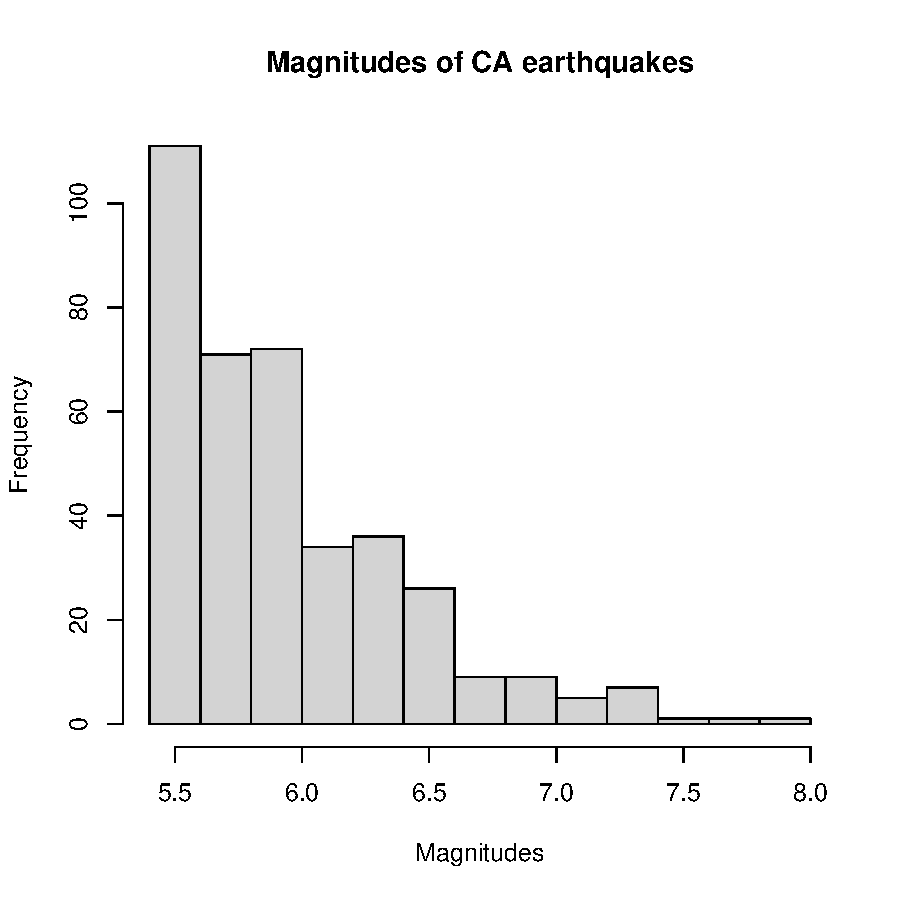
\includegraphics{RLab0_answers-038}

\begin{Schunk}
\begin{Sinput}
> #3. make plot of latitutde vs magnitude
> plot(x = CAquakes$Latitude, y = CAquakes$M, 
+      xlab = "Latitude", ylab = "Magnitude", 
+      main = "Latitude vs. Magnitude", pch = 16)
\end{Sinput}
\end{Schunk}
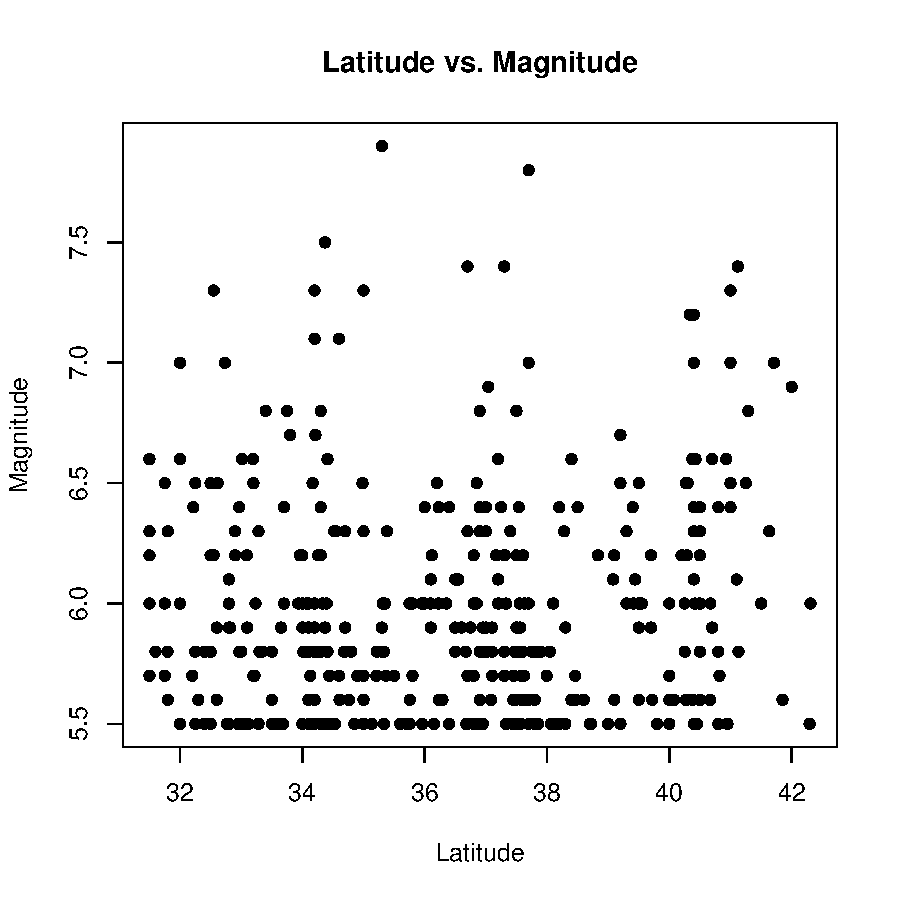
\includegraphics{RLab0_answers-039}

\end{solution}

\section{Creating functions and generating data}

There are many built-in functions in \texttt{R} (for example, above we saw the \texttt{rep()}, \texttt{seq()}, and \texttt{rnorm()} functions, to name a few). However, it's also possible to write your own functions. We will often create functions in these labs, in particular, to generate many copies of variables that comprise a dataset. The general syntax for a function is as follows:
\begin{Schunk}
\begin{Sinput}
> examplefun = function(x) { 
+   
+   y = x + 3 # what the function does
+   
+   return(y) # what we want the function to return back (output)
+ }
\end{Sinput}
\end{Schunk}

\texttt{examplefun} is the name of the function (we make that up), and \texttt{x} is the argument (input). \texttt{examplefun()} takes in as input \texttt{x}, and outputs \texttt{y}, which is the input plus 3. For example, if input 4 for \texttt{x}, we anticipate \texttt{examplefun()} to spit out 7 (i.e., 4 + 3):

\begin{Schunk}
\begin{Sinput}
> examplefun(x = 4)
\end{Sinput}
\begin{Soutput}
[1] 7
\end{Soutput}
\end{Schunk}


\noindent\textbf{On your own:}

\begin{enumerate}
\item Set the seed to 252. \\
\textit{Note:} Setting the seed to a value (generally) ensures that running the same chunk of code twice will return the exact same output, even if the code involves ``random" numbers. This will also help your GSIs help you with your labs/homework assignments/projects.
\item Create a function, \texttt{Uniform()}, that generates $n$ i.i.d. random variables uniformly distributed between 0 and $x$. \\
\textit{Hint:} the function should take in 2 arguments as input: 1) $n$, the number of uniform variables to generate, and 2) $x$, the maximum value the uniform variable can take. \textit{Extra hint:} look up the \texttt{runif()} function to randomly generate values from the uniform distribution.
\item Create a function, \texttt{generate\_data()}, that generates a dataframe with $n$ i.i.d. random variables that follow these distributions:\\
\begin{align*}
U_{W1}&\sim Uniform(0,1) \\
U_{W2}& \sim Normal(\mu=1, \sigma^2=2^2)\\
U_{A} &\sim Uniform(0,1)\\
U_{Y} &\sim Uniform(0,1)\\
\end{align*}

\textit{Hint:} the skeleton of your function should look like this (fill in the commented out parts with your own code):
\begin{Schunk}
\begin{Sinput}
> generate_data = function(n) {
+   
+   # generate n Uniform(min = 0, max = 1) variables here, set equal to U.W1
+   # generate n Normal(mean = 0, max = 1) variables here, set equal to U.W2
+   # generate n Uniform(min = 0, max = 1) variables here, set equal to U.A
+   # generate n Uniform(min = 0, max = 1) variables here, set equal to U.Y
+   
+ }
\end{Sinput}
\end{Schunk}

where \texttt{generate\_data} takes in the single argument \texttt{n}, the number of observations. Try using the \texttt{Uniform()} function you created in the previous step to generate the uniform random variables.

\item Add to the function \texttt{generate\_data()} so that it also creates 4 new variables based on the following functions that relate them:
\begin{align*}
W1&=\mathbb{I}\big[ U_{W1}<0.45 \big]\\
W2&= 0.75^*U_{W2}\\
A&=\mathbb{I}\big[ U_A < expit(-1+2.6^*W1+0.9^*W2) \big]\\
Y&=\mathbb{I}\big[ U_Y < expit(-2+A+0.7^*W1) \big] \\
\end{align*}

\emph{Hint:} Use the \texttt{as.numeric()} function for indicator variables. \\
Example: $\mathbb{I}[X > 0]$ can be coded as \texttt{as.numeric(X>0)}.

\emph{Extra hint:} Recall that the $expit$ function is the inverse of the logistic function:
\begin{align*}
logit(x) &= log\left(\frac{x}{1-x} \right)\\
expit(x) &=\frac{1}{1+e^{-x}}
 \end{align*}
In \texttt{R}, the $expit$ function is called \texttt{plogis()}.


\item Within \texttt{generate\_data()}, create a dataframe using either the \texttt{data.frame()} function or the \texttt{cbind()} function consisting of only $W1, W2, A$, and $Y$ and let that be your output (i.e., what you \texttt{return}) for the function \texttt{generate\_data()}. 

\item \textbf{Create 1000 copies of $W1, W2, A,$ and $Y$} using \texttt{generate\_data()} and set the output of the function equal to the object \texttt{ObsData}.

\item Show the first 6 lines and summary statistics of \texttt{ObsData}, using the \texttt{head()} and \texttt{summary()} functions, respectively.
\end{enumerate}

\begin{solution}

\begin{Schunk}
\begin{Sinput}
> #1. set the seed
> set.seed(252)
\end{Sinput}
\end{Schunk}
\begin{Schunk}
\begin{Sinput}
> #2. function that creates n i.i.d. uniform random variables
> Uniform = function(n, x) {
+   
+  return(runif(n = n, min = 0, max = x)) 
+ 
+ }
\end{Sinput}
\end{Schunk}
\begin{Schunk}
\begin{Sinput}
> # 3 - 5
> # function that creates n i.i.d. copies of O
> generate_data = function(n) {
+   
+   # exogenous variables
+   U.W1 = Uniform(n, x = 1)
+   U.W2 = rnorm(n, mean=1, sd=2)
+   U.A = Uniform(n, x = 1)
+   U.Y = Uniform(n, x = 1)
+   
+   # endogenous variables 
+   W1 = as.numeric( U.W1 < 0.45)
+   W2 = 0.75*U.W2
+   A = as.numeric( U.A < plogis(-1+2.6*W1+0.9*W2))
+   Y = as.numeric( U.Y < plogis(-2+A+0.7*W1))
+   
+   # dataframe with endogenous variables
+   O = data.frame(W1, W2, A, Y)
+     
+   return(O)
+ }
\end{Sinput}
\end{Schunk}
\begin{Schunk}
\begin{Sinput}
> # 6. run generate_data and set equal to ObsData dataframe
> ObsData = generate_data(1000)
\end{Sinput}
\end{Schunk}
\begin{Schunk}
\begin{Sinput}
> # 7. inspect ObsData
> head(ObsData)
\end{Sinput}
\begin{Soutput}
  W1         W2 A Y
1  0 -2.2677937 0 0
2  0  1.8953489 1 1
3  1  1.9008567 1 0
4  0  1.3315402 1 0
5  0  1.1802323 0 0
6  1 -0.4424049 1 0
\end{Soutput}
\begin{Sinput}
> summary(ObsData)
\end{Sinput}
\begin{Soutput}
       W1              W2                A               Y        
 Min.   :0.000   Min.   :-4.0304   Min.   :0.000   Min.   :0.000  
 1st Qu.:0.000   1st Qu.:-0.2148   1st Qu.:0.000   1st Qu.:0.000  
 Median :0.000   Median : 0.7559   Median :1.000   Median :0.000  
 Mean   :0.426   Mean   : 0.7803   Mean   :0.614   Mean   :0.268  
 3rd Qu.:1.000   3rd Qu.: 1.7987   3rd Qu.:1.000   3rd Qu.:1.000  
 Max.   :1.000   Max.   : 5.5581   Max.   :1.000   Max.   :1.000  
\end{Soutput}
\end{Schunk}



\end{solution}

\section{Implementation of g-computation (simple substitution estimator), IPTW, and TMLE estimation of average treatment effect of a point treatment}

Using \texttt{ObsData} we created in the previous section, we will implement g-computation, IPTW, and TMLE estimators using SuperLearner to generate estimates inspired by the average treatment effect (e.g., $\mathbb{E}[Y_{a=1} - Y_{a=0}]$). Recall from Causal I labs (note: not to worry if you don't remember much about these estimators -- we will review them [including how to implement them] later on in this course):

\begin{enumerate}
\item \textbf{Simple substitution estimator based on the G-Computation formula:} \[
\hat{\Psi}_{SS}(\hat{\mathbb{P}}) = \frac{1}{n} \sum_{i=1}^n  \big( \hat{\bar{Q}}(1, W_i) - \hat{\bar{Q}}(0, W_i) \big)
\]
where $\hat{\mathbb{P}}$ is the empirical distribution and $\hat{\bar{Q}}(A, W)$ is the estimate of the conditional mean outcome given the exposure and baseline covariates $\bar{Q}_0(A,W)\equiv \mathbb{E}_0(Y|A,W)$.\\ 
- Consistency of the simple (non-targeted) substitution estimator depends on consistent estimation of the conditional mean outcome $\bar{Q}_0(A,W)$.\\

\item \textbf{Standard (unstabilized) inverse probability weighted estimator (IPTW)}: 
\[
\hat{\Psi}_{IPTW}(\hat{\mathbb{P}}) = \frac{1}{n}\sum_{i=1}^n \left[ \frac{\mathbb{I}(A_i=1)}{\hat{g}(1|W_i)}  - 
   \frac{\mathbb{I}(A_i=0)}{\hat{g}(0|W_i)} \right] Y_i
\]
where $\hat{g}(1|W_i) = \hat{\mathbb{P}}(A_i=1|W_i)$ is an estimate of the exposure mechanism.\\
- Consistency of IPTW estimators depends on consistent estimation of the exposure mechanism $g_0(1|W) \equiv \mathbb{P}_0(A=1|W)$. \\

\begin{Schunk}
\begin{Sinput}
> predictions <- seq(0.01, 0.99, 0.01)
> weights <- 1/ predictions
> plot(weights,predictions)
\end{Sinput}
\end{Schunk}
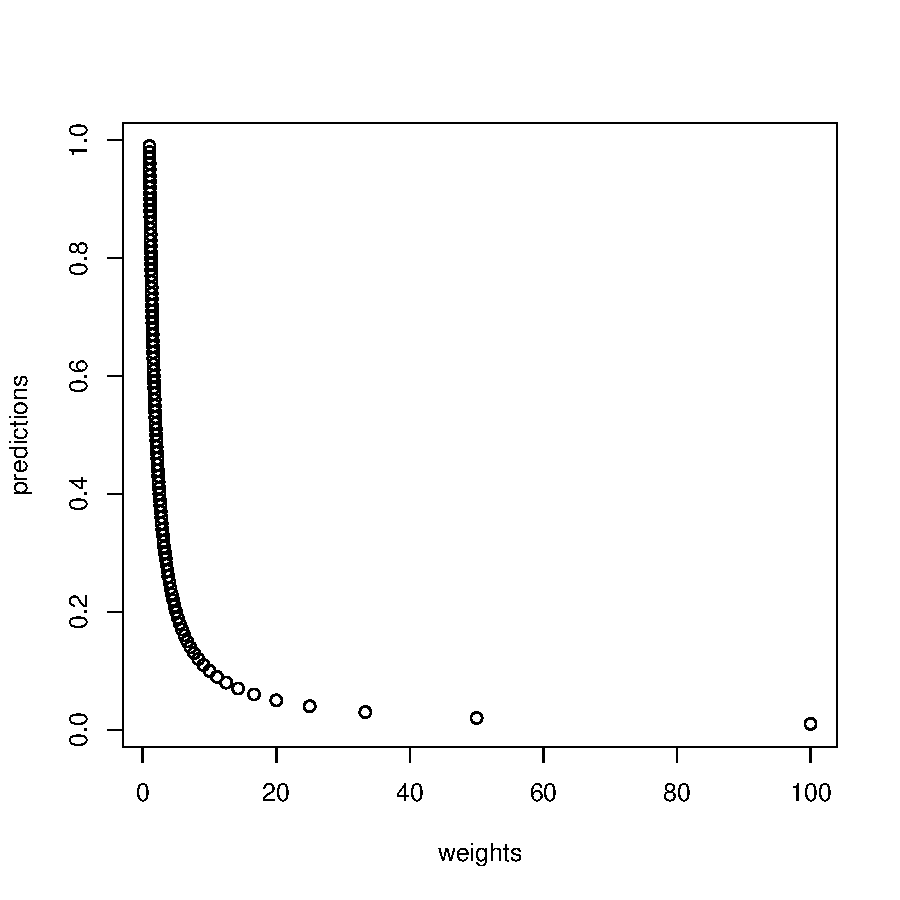
\includegraphics{RLab0_answers-048}

\item \textbf{Targeted maximum likelihood estimation (TMLE):}\[
\hat{\Psi}_{TMLE}(\hat{\mathbb{P}}) =  \frac{1}{n} \sum_{i=1}^n \big( \bar{Q}^*_n(1, W_i) - \bar{Q}^*_n(0, W_i) \big)
\]
where $\bar{Q}^*_n(A, W)$ denotes the \textit{targeted} estimate of the conditional mean outcome, given the exposure and baseline covariates $\bar{Q}_0(A,W)$.\\
- Implementation requires estimation of both the conditional mean function $\bar{Q}_0(A,W)$ and the exposure mechanism $g_0(A|W)$. \\
- Double robust estimators are consistent if {either} $\bar{Q}_0(A,W)$ {or} $g_0(A|W)$ is estimated consistently. \\
\end{enumerate}

\noindent \emph{Reminder:} An estimator is \emph{consistent} if the point estimates converge (in probability) to the estimand as sample size $n \rightarrow \infty$. \\
\noindent \emph{Reminder 2:} The notation of a subscript $n$ or hat denotes that the value is an estimate (i.e., it comes from the empirical distribution $\mathbb{P}_n$ or $\mathbb{\hat{P}}$). The notation of subscript $0$ denotes that it is a true value (i.e., the value is comes from the true population distribution, $\mathbb{P}_0$). Again, we will review this later in the course :)

\noindent \textbf{Warning:} in practice you must go through the entire roadmap to infer any causality. Here, we are simply demonstrating how to implement the estimators.

\begin{enumerate}
\item Load the \texttt{SuperLearner} and \texttt{tmle} or \texttt{ltmle} packages by using the \texttt{library()} function, and set the seed to 252.
\item Set the object \texttt{n} to the number of observations in \texttt{ObsData}. \\
\textit{Hint:} use the \texttt{nrow()} function.
\item Create a dataframe, \texttt{X}, that contains only $W1$, $W2$, and $A$ of \texttt{ObsData} \\
\textit{Hint:} use the \texttt{subset()} function.
\begin{Schunk}
\begin{Sinput}
> X = subset(ObsData, select = c(W1, W2, A))
\end{Sinput}
\end{Schunk}
\item Make new dataframes \texttt{X1} and \texttt{X0} that are copies of \texttt{X}. For the dataframe \texttt{X1}, set $A = 1$; for the dataframe \texttt{X0}, set $A = 0$. For example:
\begin{Schunk}
\begin{Sinput}
> X1$A = 1 # set A = 1 in X1 dataframe. Repeat for X0 but with A = 0.
\end{Sinput}
\end{Schunk}
\item Stack \texttt{X}, \texttt{X1}, and \texttt{X0} by using the \texttt{rbind()} function. Set the stacked data equal to the object \texttt{newdata}.
\item Set \texttt{SL.library = c('SL.glm', 'SL.mean', 'SL.glm.interaction')}. This is the SuperLearner library we'll use to estimate the outcome regression and treatment mechanism needed for the estimators.
\item \textbf{Call \texttt{SuperLearner()} to estimate $Q_0(A,W1, W2) = \mathbb{E}_0[Y|A,W1,W2]$, the outcome regression}. Specify the arguments \texttt{Y = ObsData\$Y}, \texttt{X = X}, \texttt{newX = newdata}, \texttt{SL.library = SL.library}, and \texttt{family = 'gaussian'}. Set the SuperLearner object equal to the \texttt{Qbar}.
\item Obtain the predicted/expected $Y$ given: 
\begin{enumerate}
\item the observed $A$ and covariates
\begin{Schunk}
\begin{Sinput}
> QbarAW = Qbar$SL.predict[1:n]
\end{Sinput}
\end{Schunk}
\item $A = 1$ and the observed covariates
\begin{Schunk}
\begin{Sinput}
> Qbar1W = Qbar$SL.predict[(n+1): (2*n)]
\end{Sinput}
\end{Schunk}
\item $A = 0$ and the observed covariates
\begin{Schunk}
\begin{Sinput}
> Qbar0W = Qbar$SL.predict[(2*n+1): (3*n)]
\end{Sinput}
\end{Schunk}
\end{enumerate}
\item \textbf{Evaluate the simple substituation estimator} by taking the mean of \texttt{Qbar1W} and subtracting it from the mean of \texttt{Qbar0W}:
\begin{align*}
\hat{\Psi}_{SS}(\hat{\mathbb{P}})  & = \frac{1}{n} \sum_{i=1}^n \bigg[ \hat{\mathbb{E}}(Y_i|A=1, W1_i, W2_i) - \hat{\mathbb{E}}(Y_i|A=0, W1_i, W2_i)\bigg] \\
& = \frac{1}{n} \sum_{i=1}^n \bigg[ \bar{Q}_n(1, W1_i, W2_i) - \bar{Q}_n(0, W1_i, W2_i)\bigg]
\end{align*}
\item Create a dataframe with only the covariates. Call this dataframe \texttt{W}.
\item \textbf{Call \texttt{SuperLearner()} to estimate $g_0(A|W1, W2) = P_0(A|W1, W2)$, the treatment mechanism}. Specify the arguments \texttt{Y = ObsData\$A}, \texttt{X = W}, \texttt{SL.library = SL.library}, and \texttt{family = 'binomial'}. Set the SuperLearner object equal to the \texttt{gHatSL}.
\item Generate the predicted probability of:
\begin{enumerate}
\item $A=1$ given covariates
\begin{Schunk}
\begin{Sinput}
> gHat1W = gHatSL$SL.predict
\end{Sinput}
\end{Schunk}
\item $A=0$ given covariates
\begin{Schunk}
\begin{Sinput}
> gHat0W = 1 - gHatSL$SL.predict
\end{Sinput}
\end{Schunk}
\end{enumerate}
\item \textbf{Implement the IPTW estimator} by taking a weighted average of $Y$, with weights equal to $w_i = \frac{1}{g_n(A_i|W1_i, W2_i)}$:
\begin{align*}
\hat{\Psi}_{IPTW}(\hat{\mathbb{P}})  & = \frac{1}{n}\sum_{i=1}^n \frac{\mathbb{I}(A_i=1)}{g_n(A_i|W1_i, W2_i)} Y_i - \frac{1}{n}\sum_{i=1}^n \frac{\mathbb{I}(A_i=0)}{g_n(A_i|W1_i, W2_i)} Y_i \\
& = \frac{1}{n}\sum_{i=1}^n \mathbb{I}(A_i=1)^*\hat{w}_i^*Y_i - \frac{1}{n}\sum_{i=1}^n \mathbb{I}(A_i=0)^*\hat{w}_i^*Y_i
\end{align*}
\item \textbf{Implement the TMLE estimator} by calling \texttt{tmle()} or \texttt{ltmle()}.
\begin{itemize}
\item If you're using the \texttt{tmle()} package, specify the arguments \texttt{Y = ObsData\$Y}, \texttt{A = ObsData\$A}, \texttt{W = W}, \texttt{Q.SL.library = SL.library}, \texttt{g.SL.library = SL.library}. 
\item If you're using the \texttt{ltmle()} package, specify the arguments \texttt{data=ObsData}, \texttt{Anodes='A'}, \texttt{Ynodes='Y'}, \texttt{abar=list(1,0)}, \texttt{SL.library=SL.library}. 
\end{itemize}
\end{enumerate}

\begin{solution}

\begin{Schunk}
\begin{Sinput}
> # 1. load SuperLearner and tmle packages
> library(SuperLearner)
> library(tmle)
> library(ltmle)
\end{Sinput}
\end{Schunk}
\begin{Schunk}
\begin{Sinput}
> # 2. set n equal to 1000
> n = nrow(ObsData)
\end{Sinput}
\end{Schunk}
\begin{Schunk}
\begin{Sinput}
> # 3. subset W, A and set to X
> X = subset(ObsData, select = c(W1, W2, A))
\end{Sinput}
\end{Schunk}
\begin{Schunk}
\begin{Sinput}
> # 4. create dataframes with A=1 and A=0
> X1 = X0 = X
> X1$A = 1
> X0$A = 0
\end{Sinput}
\end{Schunk}
\begin{Schunk}
\begin{Sinput}
> # 5. create newdata by stacking
> newdata = rbind(X,X1,X0)
\end{Sinput}
\end{Schunk}
\begin{Schunk}
\begin{Sinput}
> # 6. set SuperLearner library
> SL.library = c("SL.glm", "SL.mean", "SL.glm.interaction")
\end{Sinput}
\end{Schunk}
From Super Learning: An Application to the Prediction of HIV-1 Drug Resistance: 

Theoretical results show that the super learner will asymptotically outperform any of the candidate estimators it employs as long as the number of candidate learners is polynomial in sample size (or, if one of the candidate estimators it employs achieves a parametric rate of convergence, the super learner will converge at an almost parametric rate). These results suggest that the investigator pays a very small price for considering multiple alternative learners. Currently, most researchers employ one, or at most a handful, of learning algorithms to answer prediction questions. A better approach would be to apply as many candidate learners as are feasible given time and computing limitations, and choose among them using the super learner

\begin{Schunk}
\begin{Sinput}
> # 7. call superlearner to estimate E[Y|A,W]
> Qbar = SuperLearner(Y=ObsData$Y, X=X, newX=newdata, SL.library=SL.library)
\end{Sinput}
\end{Schunk}
\begin{Schunk}
\begin{Sinput}
> # 8.
> # expected Y given observed A,W
> QbarAW = Qbar$SL.predict[1:n]
> # expected Y given A=1 and W 
> Qbar1W = Qbar$SL.predict[(n+1): (2*n)]
> # expected given A=0 and W 
> Qbar0W = Qbar$SL.predict[(2*n+1): (3*n)]
\end{Sinput}
\end{Schunk}
\begin{Schunk}
\begin{Sinput}
> # 9.
> ### Simple substitution estimator of the ATE ###
> PsiHat.SS = mean(Qbar1W - Qbar0W)
\end{Sinput}
\end{Schunk}
\begin{Schunk}
\begin{Sinput}
> # 10. create dataframe of covariates
> W = subset(X, select = c(W1, W2))
\end{Sinput}
\end{Schunk}
\begin{Schunk}
\begin{Sinput}
> # 11. call superlearner to estimate g_0(A|W)
> gHatSL = SuperLearner(Y=ObsData$A, X=W, SL.library=SL.library, family="binomial")
\end{Sinput}
\end{Schunk}
\begin{Schunk}
\begin{Sinput}
> # 12.
> # generate the predicted prob A=1, given baseline cov
> gHat1W = gHatSL$SL.predict
> # generate the predicted prob of A=0, given baseline cov
> gHat0W = 1 - gHatSL$SL.predict
\end{Sinput}
\end{Schunk}
\begin{Schunk}
\begin{Sinput}
> # 13.
> ### IPTW estimator of the ATE ###
> IPTW_comps <- cbind(ObsData$A, gHat1W,ObsData$A/gHat1W,  gHat0W, (1-ObsData$A)/gHat0W, ObsData$Y)
> colnames(IPTW_comps) <- c("A", "Predict A = 1", " A = 1 Weight", "Predict A = 0", "A = 0 weight", "Outcome")
> head(IPTW_comps)
\end{Sinput}
\begin{Soutput}
  A Predict A = 1  A = 1 Weight Predict A = 0 A = 0 weight Outcome
1 0    0.04424412      0.000000    0.95575588     1.046292       0
2 1    0.67537229      1.480665    0.32462771     0.000000       1
3 1    0.96175256      1.039768    0.03824744     0.000000       0
4 1    0.55196392      1.811713    0.44803608     0.000000       0
5 0    0.51698380      0.000000    0.48301620     2.070324       0
6 1    0.74813608      1.336655    0.25186392     0.000000       0
\end{Soutput}
\begin{Sinput}
> PsiHat.IPTW = mean(ObsData$A*ObsData$Y/gHat1W) - 
+   mean((1-ObsData$A)*ObsData$Y/gHat0W)
\end{Sinput}
\end{Schunk}
\begin{Schunk}
\begin{Sinput}
> # 14.
> ### TMLE of ATE ###
> PsiHat.TMLE_tmle = tmle(Y = ObsData$Y, A = ObsData$A, W = W, 
+                         Q.SL.library = SL.library, g.SL.library = SL.library)
> PsiHat.TMLE_ltmle = summary(ltmle(data=ObsData, Anodes='A', Ynodes='Y', 
+                           abar=list(1,0), SL.library=SL.library))
> PsiHat.SS
\end{Sinput}
\begin{Soutput}
[1] 0.1139461
\end{Soutput}
\begin{Sinput}
> PsiHat.IPTW
\end{Sinput}
\begin{Soutput}
[1] 0.114629
\end{Soutput}
\begin{Sinput}
> PsiHat.TMLE_ltmle$effect.measures$ATE
\end{Sinput}
\begin{Soutput}
$long.name
[1] "Additive Treatment Effect"

$estimate
[1] 0.08336901

$std.dev
[1] 0.05282814

$pvalue
[1] 0.1145386

$CI
            2.5%     97.5%
[1,] -0.02017223 0.1869103

$log.std.err
[1] FALSE
\end{Soutput}
\begin{Sinput}
> PsiHat.TMLE_tmle$estimates$ATE
\end{Sinput}
\begin{Soutput}
$psi
[1] 0.08220612

$var.psi
[1] 0.002418168

$CI
[1] -0.01417662  0.17858887

$pvalue
[1] 0.09458152
\end{Soutput}
\end{Schunk}

\end{solution}

\vfill 
\noindent Lab Adapted from Spring 2015 Stat 133 Lab and Lecture by Deborah Nolan, Chris Paciorek's 2014 R bootcamp, Causal I Lab 0 by Alex Leudtke


\end{document}


